\chapter[Nuclear Reactions in Stars]{\textbf{Nuclear Reactions \\ in Stars}}
\label{ch:reactions}

\section{Introduction}

% I might not need an introduction section, but keep for now.

This chapter introduces the formalism for quantifying stellar nucleosynthesis with reaction rates, which is an important foundation for the rest of this thesis. Section \ref{sec:nuc_reac_network} introduces the concept of a nuclear reaction network, involving the abundance evolution of each nucleus given all possible reactions in the network. Section \ref{sec:rates} describes the formalism for reaction rate calculations, with a focus on resonant reactions. Finally, Section \ref{sec:transfer_reactions} will describe the theory of transfer reactions, and their use in obtaining experimental information on the key nuclear structure inputs for reaction rates.

%%%%%%%%%%%%%%%%%%%%%%%%%%%%%%%%%%%%%%%%%%%%%%%%%%%%%%%%%%%%%%%%%%%%%%%%%%%%%%%%%%%%%%%%%%%%%

\section{Nuclear Reaction Networks} \label{sec:nuc_reac_network}

% Equation from Christian's book that adds the production reactions and subtracts the destruction reactions, involving the reaction rates

Nuclei in a high temperature stellar plasma are constantly undergoing nuclear processes, changing the overall composition of the stellar region. Each nucleus has several possible ways in which it can be destroyed and produced, depending on the environmental conditions and stellar composition at any given time. To quantify the change in abundance of a given nuclear species, we track its number density $N(t)$ over time, as introduced in Equation \ref{eqn:sProcess_AbundEvol}. Here, we will obtain a general expression for the abundance evolution of any nuclear species. To derive the expression, first consider the reaction between two nuclei 0 and 1. The rate at which this reaction proceeds is related to the mean lifetime $\tau$, or inversely, the decay constant $\lambda \equiv 1/\tau$ of the nuclear species in the stellar plasma. The rate of change of $N_{0}(t)$ over time from reactions with nucleus 1 is expressed as
\begin{equation} \label{eqn:AbundEvol_01}
\left( \frac{dN_{0}}{dt} \right)_{1} = -\lambda_{1}(0)N_{0} = - \frac{N_{0}}{\tau_{1}(0)} = N_{0}N_{1}\langle \sigma v \rangle_{01},
\end{equation}
where $\langle \sigma v \rangle_{01}$ is the reaction rate for a single pair of particles 0 and 1. The number density for species $i$ can also be written as $N_{i} = \rho X_{i} N_{A} / M_{i}$, where $\rho$ is the mass density of the stellar plasma, $X_{i}$ and $M_{i}$ are the mass fraction and mass of species $i$, respectively, and $N_{A}$ is Avogadro's number. Hence, the decay constant for nucleus 1 can also be expressed as
\begin{equation} \label{eqn:decay_constant}
\lambda_{1}(0) = \frac{1}{\tau_{1}(0)} = N_{1} \langle \sigma v \rangle_{01} = \rho \frac{X_{1}}{M_{1}} N_{A} \langle \sigma v \rangle_{01}.
\end{equation}
Eqn. \ref{eqn:decay_constant} is used frequently to determine the preferred reaction by which a nucleus is destroyed in a stellar plasma \cite{Iliadis2015}. In the s-process, for example, it can be used to determine which branch of an s-process branching will be preferred, or if the paths have roughly equal probability. In hydrogen-burning nucleosynthesis, it can be used to determine if a burning cycle will be closed or if it will be escaped. Note that the decay constant depends on both the stellar mass density and temperature, the latter of which through $\langle \sigma v \rangle$.

Now consider every nuclear process that can occur on a given nuclear species $i$, including nuclear reactions, photoabsoptions, and $\beta$-decays. In the absence of mixing and expansion, its net abundance evolution is expressed by the differential equation\footnote{If nonidentical particles $j$ and $k$ produce two nuclei $i$, then the first term in Eqn. \ref{eqn:AbundEvol_General} must be replaced by $2N_{j}N_{k}\langle \sigma v \rangle_{jk \rightarrow i}$. If identical particles $(j = k)$ produce only one nucleus $i$, then that term must instead be replaced by $N_{j}^{2}\langle \sigma v \rangle_{jj \rightarrow i}/2$. Analogous arugments apply to the fourth term.}
\begin{align}
\frac{dN_{i}}{dt} = &\sum_{j,k} N_{j}N_{k} \langle \sigma v \rangle_{jk \rightarrow i} + \sum_{l} \lambda_{\beta, l \rightarrow i} N_{l} + \sum_{m} \lambda_{\gamma, m \rightarrow i} N_{m} \nonumber \\
&- \sum_{n} N_{n}N_{i}\langle \sigma v \rangle_{ni} - \sum_{o} \lambda_{\beta, i \rightarrow o} N_{i} - \sum_{p} \lambda_{\gamma, i \rightarrow p} N_{i}. \label{eqn:AbundEvol_General}
\end{align}
The terms in the first and second lines represent all possible production and destruction processes, respectively, for the nuclear species $i$. The first term includes all reactions between nuclei $j$ and $k$ producing nucleus $i$; the second term includes all nuclei $l$ $\beta$-decaying to nucleus $i$; the third term includes all photoabsorption reactions on nuclei $m$ leading to nucleus $i$, and the remaining terms represent the analogous, reverse destruction processes.

In order to properly describe nucleosynthesis in a stellar plasma, we must account for the abundance evolution of all relevant nuclei in the environment, each described by Eqn. \ref{eqn:AbundEvol_General}. This system of coupled, nonlinear ordinary differential equations is known as a \emph{nuclear reaction network}. In most realistic scenarios, this system of equations must be solved numerically. The number density $N_{i}(t)$ of each nucleus in the network is typically given in terms of the mass fraction $X_{i}(t)$, where $\sum_{i} X_{i}(t) = 1$, as it is much simpler to conceptualize relative mass fractions than number densities. Solutions to the nuclear reaction network at some final time $t_{f}$ are therefore reported as final mass fractions $X_{f}$ and are nominally referred to as final abundances. From $N_{i} = \rho X_{i} N_{A} / M_{i}$, the mass fraction normalization can be expressed as
\begin{equation}
\sum_{i} X_{i} = \sum_{i} \frac{N_{i}M_{i}}{\rho N_{A}} = 1.
\end{equation}
Hence, $\rho N_{A} = \sum_{i} N_{i}M_{i}$, and the mass fraction can therefore be written as
\begin{equation} \label{eqn:mass_fraction}
X_{i} = \frac{N_{i}M_{i}}{\sum_{i} N_{i}M_{i}} \approx \frac{N_{i}A_{i}}{\sum_{i} N_{i}A_{i}},
\end{equation}
where the nuclear masses $M_{i}$ can usually be approximated by the mass number $A_{i}$. Eqn. \ref{eqn:mass_fraction} is especially convenient when considering, for example, a network consisting of initially solar system abundances, such as that of Ref. \cite{Lodders2009}. These solar system number densities $N$ are normalized to $10^{6}$ Si atoms, and relative isotopic abundances are taken into account. When putting these $N$-values into Eqn. \ref{eqn:mass_fraction}, this normalization cancels. Often the network is selected from a subset of solar system nuclei, in which case it is a simple matter of adjusting the mass fractions so that their sum remains unity. Even in cases where some of the solar system abundances should be modified to represent a specific stellar environment, as will be the case in Section \ref{subsec:reaction_network_sProcess}, Eqn. \ref{eqn:mass_fraction} makes this scenario trivial.

%In this thesis, nuclear reaction network calculations are performed at constant mass density $\rho$ and temperature $T$.

\section{Reaction Rates} \label{sec:rates}

The reaction rate per particle pair in a stellar medium is given by
\begin{equation} \label{eqn:reaction_rate}
\left\langle \sigma v \right\rangle_{01} = \sqrt{\frac{8}{\pi \mu_{01}}} \, \frac{1}{(kT)^{3/2}} \int_{0}^{\infty} E \, \sigma(E) \, e^{-E/kT} \, dE,
\end{equation}
where $\mu_{01}$ is the reduced mass of particle 0 and particle 1, $\mu = M_{0}M_{1}/(M_{0}+M_{1})$; $k$ is the Boltzmann constant; $T$ is the stellar temperature; $E$ is the center-of-mass energy between the particles; and $\sigma(E)$ is the reaction cross section evaluated at $E$. The energy dependence of the cross section determines whether numerical integration must be performed. The formalism for reaction rate calculations therefore depends on whether $\sigma(E)$ is smoothly varying over energy (for non-resonant reactions) or if it can be described by isolated resonances (for resonant reactions). It can be described by both in principle, in which case the cross section is separated into non-resonant and resonant components, assuming interference effects are negligible. Regardless of the nature of $\sigma(E)$, it can be separated into a Coulomb factor and a factor resulting only from nuclear structure. That is, the cross section can be rewritten as
\begin{equation} \label{eqn:S-factor}
\sigma(E) = \frac{1}{E} \, e^{-2 \pi \eta} \, S(E),
\end{equation}
where $S(E)$ is the astrophysical S-factor, governed by nuclear effects alone, and $\eta$ is the Sommerfeld parameter defined by $2 \pi \eta = \sqrt{2 \mu_{01} / E} \,  Z_{0} Z_{1} e^{2} / \hbar$, where $Z_{0}$ and $Z_{1}$ are the atomic numbers of the nuclei. The $1/E$ factor is included to cancel with the $E$ factor in the reaction rate. Substituting Eqn. \ref{eqn:S-factor} into Eqn. \ref{eqn:reaction_rate}, we have
\begin{equation} \label{eqn:reaction_rate_S-factor}
\left\langle \sigma v \right\rangle_{01} = \sqrt{\frac{8}{\pi \mu_{01}}} \, \frac{1}{(kT)^{3/2}} \int_{0}^{\infty} e^{-2 \pi \eta} \, e^{-E/kT} \, S(E) \, dE.
\end{equation}

The integrand in Eqn. \ref{eqn:reaction_rate_S-factor} is composed of the Gamow factor $e^{-2 \pi \eta}$, the Maxwell-Boltzmann factor $e^{-E/kT}$, and the astrophysical S-factor $S(E)$. The former two factors have a combined energy dependence of $e^{-\sqrt{1/E}} \, e^{-E}$, while the $S(E)$ energy dependence is based on the nuclear structure of the specific reaction. The overlap between the Gamow and Maxwell-Boltzmann factors is called the \emph{Gamow peak}, $e^{-2 \pi \eta} \, e^{-E/kT}$. This peak determines the energies at which the reaction will proceed in the stellar environment at the given temperature\footnote{This is a slight oversimplification. For resonant reactions at high stellar temperatures, the resonances that contribute significantly to the reaction rate may occur below the Gamow peak \cite{Iliadis2015}.}. It has a maximum at
\begin{align}
E_{0} &= \left[ \left(\frac{\pi}{\hbar}\right)^{2} (Z_{0} Z_{1} e^{2})^{2} \left(\frac{m_{01}}{2}\right) (kT)^{2} \right]^{1/3} \nonumber \\
&= 0.1220 \left(Z_{0}^{2} Z_{1}^{2} \mu_{01} T_{9}^{2} \right)^{1/3} \,\, [\mathrm{MeV}]
\end{align}
where $T_{9}$ is the temperature in units of GK. The energy $E_{0}$ is the most probable energy for non-resonant reactions, where $S(E)$ varies smoothly. For resonant reactions, where $S(E)$ is described by a sharp Lorentzian function, the Gamow peak can still be a useful indicator of which resonances contribute significantly to the total reaction rate, particularly at lower resonance energies ($E_{r}^{\mathrm{c.m.}} \lesssim 0.5$ MeV). The Gamow peak can be approximated by a Gaussian function with a mean of $E_{0}$ and a $1/e$ width of
\begin{equation}
\Delta = \frac{4}{\sqrt{3}} \sqrt{E_{0} k T} = 0.2368 \left(Z_{0}^{2} Z_{1}^{2} \mu_{01} T_{9}^{5}\right)^{1/6} \,\, [\mathrm{MeV}].
\end{equation}
Thermonuclear reactions therefore mainly occur in the energy window from $E_{0} - \Delta/2$ to $E_{0} + \Delta/2$, known as the \emph{Gamow window}.

For the $^{39}\mathrm{K}(p,\gamma)^{40}\mathrm{Ca}$ reaction, discussed in Chapter \ref{ch:GC}, the Gamow window at temperatures of 100 MK occurs between about 140 keV and 230 keV, centered on about 185 keV. This situation is depicted in Figure \ref{fig:Gamow_Window}. The Gamow and Maxwell-Boltzmann factors are shown in red and green, respectively, while the combined Gamow peak is shown in blue. The Gamow window centered on $E_{0}$ is shown between the vertical dotted lines. As will be clear in Section \ref{subsec:resonance_contributions}, the $^{39}\mathrm{K}(p,\gamma)^{40}\mathrm{Ca}$ reaction rate is dominated by isolated resonances in the temperature range of astrophysical interest, 80--260 MK, occuring between about 120 keV and 450 keV.

\begin{figure}[t]
\begin{tikzpicture}
\node at (0,0) {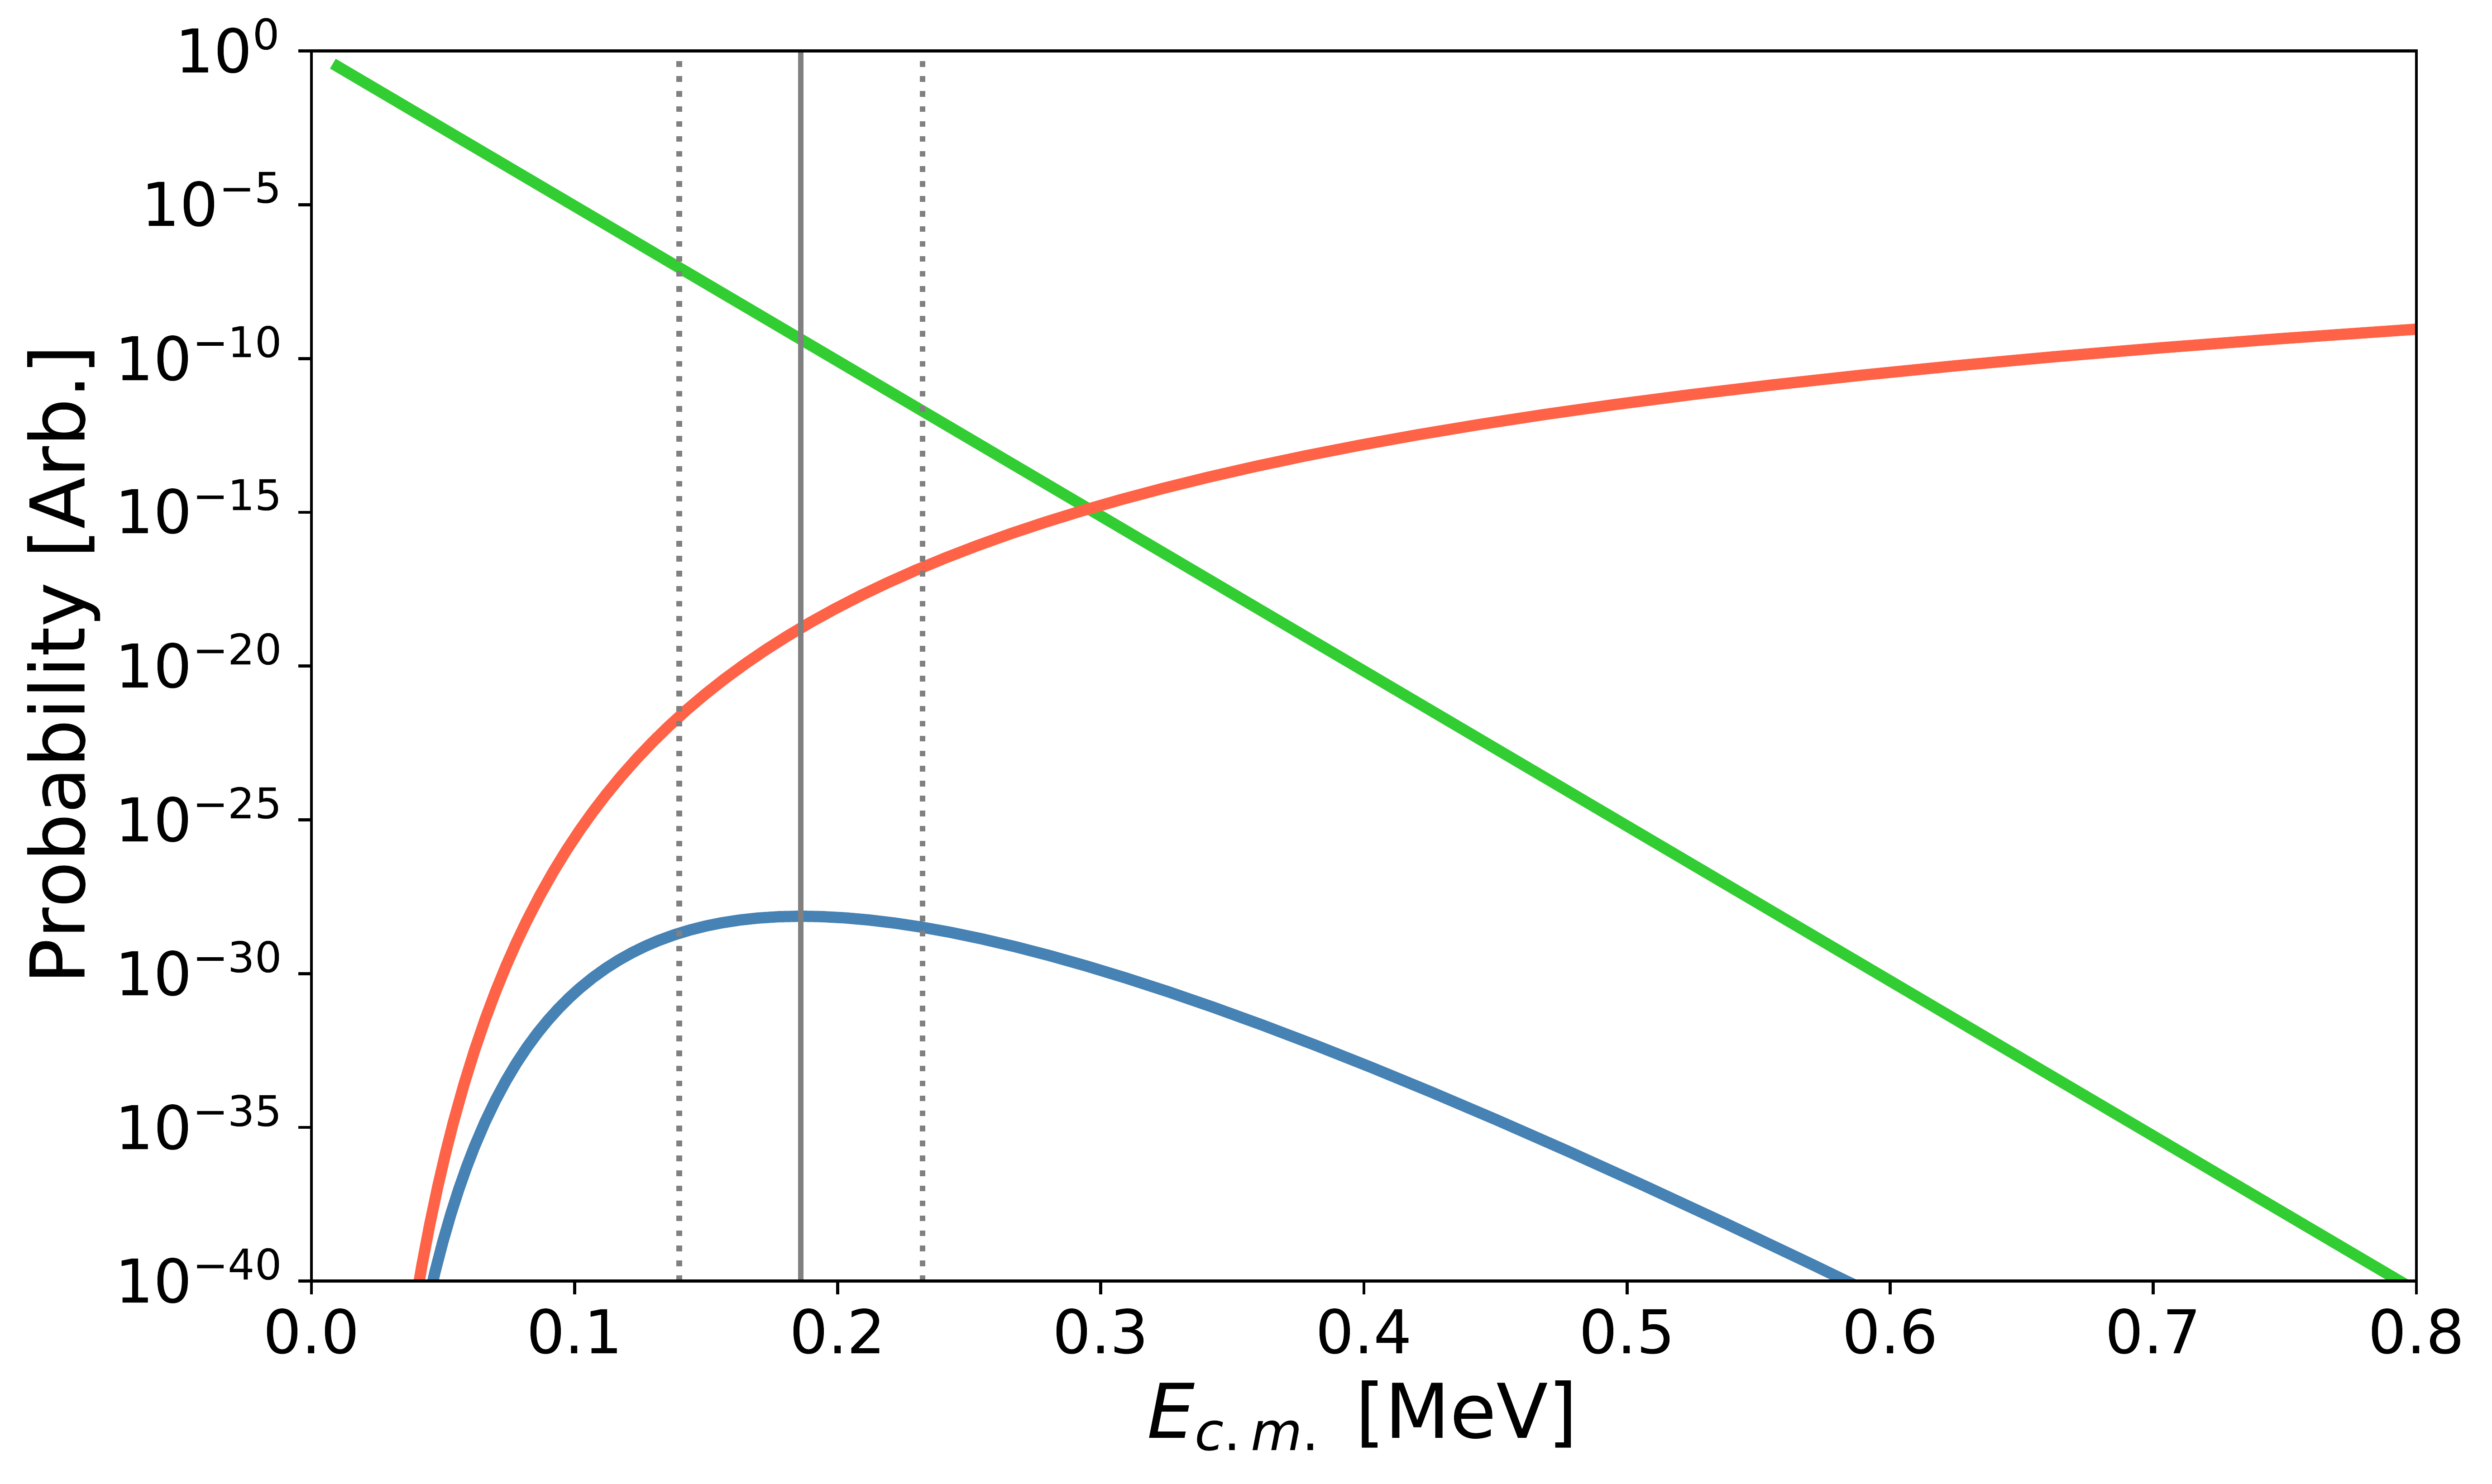
\includegraphics[width=6.5in]{Chapter-2/figs/Gamow_Window.png}};
\node at (5,3.15) {\Huge{$e^{-2\pi\eta}$}};
\node at (5,-0.5) {\Huge{$e^{-E/kT}$}};
\node[rotate=-20] at (1,-1.575) {\Huge{$e^{-2\pi\eta} e^{-E/kT}$}};
\node at (-5,2) {\large{$E_{0} \pm \frac{\Delta}{2}$}};
\draw[line width = 0.1 mm] (-4.9,1) -- (-3,1);
\draw[>=triangle 45, line width = 0.1 mm, ->] (-4.9,1) -- (-4.9,1.7);
\node at (0.5,3.9) (A) {\large{$T = 100$ MK}};
\node[draw=black, fit=(A)] {};
\end{tikzpicture}
\caption{\label{fig:Gamow_Window}The Gamow window, $E_{0} \pm \Delta/2$, for the $^{39}\mathrm{K}(p,\gamma)^{40}\mathrm{Ca}$ reaction at 100 MK. The Gamow factor $e^{-2 \pi \eta}$ is shown in red; the Maxwell-Boltzmann factor $e^{-E/kT}$ is shown in green, and the Gamow peak $e^{-2 \pi \eta} e^{-E/kT}$ is shown in blue. The resonances that contribute significantly to the reaction rate at this temperature will have energies within the Gamow window, between about 140 keV and 230 keV.}
\end{figure}

\subsection{Narrow Resonances} \label{subsec:narrow_resonances}

An isolated resonance at the resonance energy $E_{r}$ is described by the Breit-Wigner cross-section \cite{Breit1936}
\begin{equation} \label{eqn:BW_Cross}
\sigma_{\mathrm{BW}}(E) = \frac{\lambda^{2}}{4 \pi} \, \omega \frac{\Gamma_{a}(E) \, \Gamma_{b}(E)}{\left(E - E_{r}\right)^{2} + \Gamma(E)^{2}/4},
\end{equation}
where $\lambda$ is the deBroglie wavelength, defined by $\lambda^{2}/2 = (\pi \hbar)^{2} / (\mu_{01} E)$; $\Gamma_{a}(E)$ and $\Gamma_{b}(E)$ are the entrance channel and exit channel partial widths, respectively; $\Gamma(E)$ is the total width, and $\omega$ is the spin factor, defined as
\begin{equation}
\omega = \frac{(2J+1)}{(2J_{0}+1) (2J_{1}+1)},
\end{equation}
where $J$ is the resonance spin, and $J_{0}$ and $J_{1}$ are the spins of the interacting particles. Substituting Eqn. \ref{eqn:BW_Cross} into Eqn. \ref{eqn:reaction_rate}, the reaction rate per particle pair arising from an isolated resonance becomes
\begin{equation}
\left\langle \sigma v \right\rangle_{01} = \frac{\sqrt{2 \pi} \hbar^{2}}{\left(\mu_{01} k T\right)^{3/2}} \, \omega \int_{0}^{\infty} \frac{\Gamma_{a}(E) \, \Gamma_{b}(E)}{\left(E - E_{r}\right)^{2} + \Gamma(E)^{2}/4} \, e^{-E/kT} \, dE.
\end{equation}

Consider the partial widths $\Gamma_{i}$ and the Maxwell-Boltzmann factor $e^{-E/kT}$ varying slowly with energy over the width of the resonance. In this situation, the resonance is considered narrow, and these factors can be treated as being independent of energy over this energy range. The reaction rate is then written as
\begin{align}
\left\langle \sigma v \right\rangle_{01} &= \frac{\sqrt{2 \pi} \hbar^{2}}{\left(\mu_{01} k T\right)^{3/2}} \, \omega \Gamma_{a} \, \Gamma_{b} \, e^{-E_{r}/kT} \int_{0}^{\infty} \frac{dE}{\left(E - E_{r}\right)^{2} + \Gamma(E)^{2}/4} \nonumber \\
&= \frac{\sqrt{2 \pi} \hbar^{2}}{\left(\mu_{01} k T\right)^{3/2}} \, \omega \Gamma_{a} \, \Gamma_{b} \, e^{-E_{r}/kT} \, \frac{2}{\Gamma} \, \left. \arctan\left( \frac{E - E_{r}}{\Gamma/2} \right)\right|_{0}^{\infty} \nonumber \\
&= \left(\frac{2 \pi}{\mu_{01} k T}\right)^{3/2} \hbar^{2} \, \omega \frac{\Gamma_{a} \, \Gamma_{b}}{\Gamma} \, e^{-E_{r}/kT},
\end{align}
where the last line results from the further approximation of narrow resonances, $E_{r} >> \Gamma$, which makes the lower bound of integration effectively $-\infty$. The quantity
\begin{equation}
\omega \gamma \equiv \omega \frac{\Gamma_{a} \, \Gamma_{b}}{\Gamma}
\end{equation}
is defined as the \emph{resonance strength} because it is proportial to the maximum cross section multiplied by the total resonance width, $\omega \gamma \propto \sigma_{\mathrm{max}} \Gamma$. The reaction rate per particle pair for multiple isolated, narrow resonances forms an incoherent sum,
\begin{equation}
\left\langle \sigma v \right\rangle_{01} = \left(\frac{2 \pi}{\mu_{01} k T}\right)^{3/2} \hbar^{2} \, \sum_{i} \, (\omega \gamma)_{i} \, e^{-E_{r, \, i}/kT}.
\end{equation}
The calculation of partial widths differs between particles and $\gamma$-rays. The following discussion will consider charged-particles and $\gamma$-rays only. For a discussion of neutron partial widths, see Ref. \cite{Iliadis2015}.

\subsection{Particle Partial Widths}

The charged-particle partial width for channel $c$ is
\begin{equation} \label{eqn:partial_width}
\Gamma_{c}(E) = \frac{2 \hbar^{2}}{\mu_{01} R^{2}} \, P_{c}(E) \, C^{2}S \, \theta_{\mathrm{sp}, \, c},
\end{equation}
where the channel radius $R$ is defined by $R = R_{0} \left( A_{0}^{1/3} + A_{1}^{1/3} \right)$; the penetration factor $P_{c}(E)$ can be calculated as
\begin{equation}
P_{c}(E) = \frac{\rho}{F^{2}(E) + G^{2}(E)},
\end{equation}
where $\rho = 0.21874 \, R \, \sqrt{\mu_{01} E}$ and $F$ and $G$ are the energy dependent Coulomb wave functions; $C^{2}S$ is the spectroscopic factor, sometimes simply referred to as $S$, where $C$ is the isospin Clebsch-Gordon coefficient, and $\theta_{\mathrm{sp}, \, c}$ is the dimensionless single-particle reduced width. The charged-particle partial width can be thought of as being proportional to the probability of the particle being emitted from the compound nucleus. Each of the latter three quantities in Eqn. \ref{eqn:partial_width} contribute to this probability. The penetration factor $P_{c}(E)$ represents the probability of overcoming or tunneling through the Coulomb barrier to reach the nuclear surface. The dimensionless single-particle reduced width $\theta_{\mathrm{sp}, \, c}$ represents the probability that the particle occupies the exact single-particle shell-model state of the resonance at the nuclear surface. Finally, the spectroscopic factor $C^{2}S$ is a measure of how much the populated state resembles that single-particle shell-model state. Although $C^{2}S$ is model-dependent, it is the only quantity in Eqn. \ref{eqn:partial_width} that is based on measurement, as will be clear in Section \ref{subsec:DWBA}.

The dimensionless single-particle reduced width is given by
\begin{equation}
\theta_{\mathrm{sp}, \, c} = \frac{R}{2} | u_{\mathrm{sp}, \, c}(R) |^{2},
\end{equation}
where $u_{\mathrm{sp}, \, c}(R)$ is the single-particle radial wavefunction evaluated at the channel radius, which is normalized to unity as in
\begin{equation}
\int_{0}^{R} |u_{\mathrm{sp}, \, c}(R)|^{2} \, r^{2} \, dr = 1.
\end{equation}
One method of numerically calculating $\theta_{\mathrm{sp}, \, c}$ is to vary the parameters of the single-particle potential until a resonance is produced at the binding energy. This is performed, for example, by the code \texttt{BIND}, detailed in Ref. \cite{Iliadis1997}. Another procedure, performed for $^{39}\mathrm{K}(p, \gamma)^{40}\mathrm{Ca}$ in Sec. \ref{subsec:partial_widths}, is to use the weak binding approximation. This approximation is required if the nuclear reaction code used in the determination of $C^{2}S$ only handles bound states, as is the case with \texttt{Fresco} \cite{Thompson1988,Fresco}. This method assumes unbound states are weakly bound (by $\lesssim 50$ keV), and therefore $u_{\mathrm{sp}, \, c}(R)$ is the bound state radial wavefuction evaluated at the channel radius. The channel radius $R$ is selected to represent the nuclear surface, where the wavefunctions for the bound state and unbound state are equivalent.

A fact that appears troubling for the weak binding approximation at first glance is that both $C^{2}S$ and $\theta_{\mathrm{sp}, \, c}$ depend linearly on the binding energy, assuming $R$ is chosen at the nuclear surface. Therefore, both quantities will diverge from unbound calculations at high binding energies. However, as Ref. \cite{Harrouz2023} has shown for the proton-transfer reaction $^{30}\mathrm{Si}(^{3}\mathrm{He},d)^{31}\mathrm{P}$, $C^{2}S$ decreases as a function of binding energy at roughly the same rate as $\theta_{\mathrm{sp}, \, c}$ increases, such that their product is balanced. The only signficant energy dependence from Eqn. \ref{eqn:partial_width} therefore comes from the penetration factor $P_{c}(E)$, which can easily be evaluated for unbound energies without the use of the weak binding approximation.

\subsection{$\gamma$-ray Partial Widths}
The $\gamma$-ray partial width for a single transition is
\begin{equation}
\Gamma_{\gamma}(\bar{\omega}, E_{\gamma}) = \frac{8 \pi (L + 1)}{L\left[(2L + 1)!!\right]^{2}} \left(\frac{E_{\gamma}}{\hbar c}\right)^{2L+1} B(\bar{\omega}L),
\end{equation}
where $\bar{\omega}$ represents either electric or magnetic radiation; $E_{\gamma}$ is the $\gamma$-ray transition energy; $L$ is the $\gamma$-ray multipolarity, and $B$ is the branching ratio. The $\gamma$-ray partial width at the incoming particle energy $E$ can be scaled with respect to that of the resonance energy $E_{r}$ as in
\begin{equation}
\Gamma_{\gamma}(E) = \Gamma_{\gamma}(E_{r}) \left(\frac{E + Q - E_{f}}{E_{r} + Q - E_{f}}\right)^{2L+1},
\end{equation}
where $Q$ is the $Q$-value, or equivalently, the particle separation energy, and $E_{f}$ is the final excitation energy of the $\gamma$-decay.

%%%%%%%%%%%%%%%%%%%%%%%%%%%%%%%%%%%%%%%%%%%%%%%%%%%%%%%%%%%%%%%%%%%%%%%%%%%%%%%%%%%%%%%%%%%%%
\section{Transfer Reactions} \label{sec:transfer_reactions}

% This will be the last section of this chapter
% Theory leading to C2S definition from overlap functions
% And C2S from DWBA and experimental cross section

\subsection{Optical Model} \label{subsec:Optical_Model}



\subsection{Distorted Wave Born Approximation} \label{subsec:DWBA}

% Theoretical model, similar to Caleb's Section in his Chapter 2

% For a surface level explanation (good for defense questions! and for intro to section), see Krane pg. 421-424.

% Include Zero-range approximation

%\subsection{Spectroscopic Factors} \label{subsec:C2S}
% Might not need this section (should be covered in both Narrow Resonance and DWBA sections)
%\subsection{Proton Partial Widths} \label{subsec:PartialWidths}
% Might not need this section (should be covered in Narrow Resonance section)